\graphicspath{{lectures/06_eloadas_abrak/}}

\section{Elsőrendű lineáris egyenletek, Bernoulli-típusú egyenletek és lineáris rendszerek}

\subsection{Az előző előadásból folytatott egyenlettípus}
Az előző. előadás végén szereplő, homogén fokszámú egyenletre vezető feladat
folytatása (2019. 10. 16.):
\begin{align*}
  u(t)&:=\frac{x(t)}{t}
  &&\Longrightarrow\quad x(t)=t\,u(t)\\
  &\Longrightarrow\quad
  x'(t)=u(t)+t\,u'(t)=f(u(t))\\
  &\Longrightarrow\quad
  u'(t)=\frac{1}{t}\bigl(f(u(t))-u(t)\bigr).
\end{align*}
Ez szétválasztható differenciálegyenlet.

\textbf{1. megjegyzés.}
A jobb oldaltól függő új függvény bevezetésével lehet próbálkozni
(lásd a Kamke-könyvet).

\textbf{2. megjegyzés.}
Figyelni kell a jobb oldal értelmezési tartományára ($D_f$-re).

\subsection{Elsőrendű lineáris differenciálegyenletek}
\textit{Kéziratos hivatkozás: „L: An. alk. 6. ea.”}

\textbf{Általános alak.} Adott $I\subseteq\mathbb R$ nyílt intervallum,
$f,g:I\longrightarrow\mathbb R$ folytonos függvények. Az egyenlet:
\[
 x'(t)+f(t)x(t)=g(t),\qquad t\in I.
\]
A hozzá tartozó kezdetiérték-probléma:
\[
 (\tau,\xi)\in I\times\mathbb R,
 \qquad x(\tau)=\xi.
\]

\begin{center}
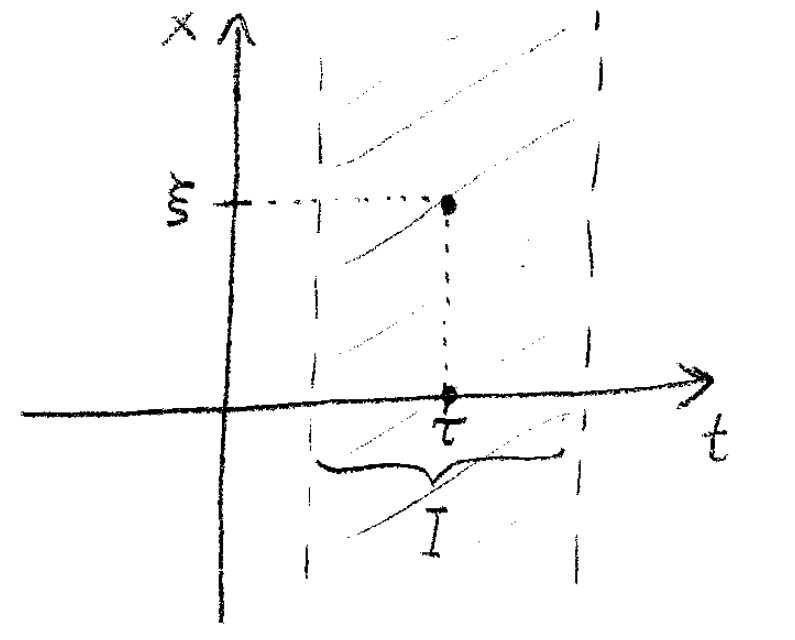
\includegraphics[width=0.37\linewidth]{01_linearis_kezdeti_ertek_tartomany.png}
\figlabel{Az $I$ intervallum és a $(\tau,\xi)$ kezdeti adat az eredeti kézirat 19. PDF-oldalán.}
\end{center}

\subsubsection*{1. módszer: integrálótényezővel}
Tegyük fel, hogy $\varphi$ a kezdetiérték-probléma megoldása,
$J\subseteq I$ nyílt intervallumon. Ekkor
\[
 \varphi'(t)+f(t)\varphi(t)=g(t).
\]
Szorozzunk az $\displaystyle e^{\int_\tau^t f}$
integrálótényezővel, amely pozitív:
\[
 e^{\int_\tau^t f}>0.
\]
A szorzat deriválásával
\[
 \left(\varphi(t)\,e^{\int_\tau^t f}\right)'
 =e^{\int_\tau^t f}\,g(t),\qquad t\in J.
\]
A $\varphi(\tau)=\xi$ kezdeti feltételből következik:
% FORRÁSHŰ: a 20. kéziratoldalon a jobb oldali belső integrál felső határa t.
% Ennek matematikai lehetséges javítását lásd: ellenorzes.md.
\[
 \varphi(t)e^{\int_\tau^t f}-\xi
 =\int_\tau^t e^{\int_\tau^t f}\,g(s)\,ds,
 \qquad t\in J.
\]
Ekkor $J=I$ is vehető. Tehát a kezdetiérték-probléma
\textbf{globálisan egyértelműen oldható meg}.

A teljes megoldás értelmezési tartománya $I$.

\subsubsection*{2. módszer: homogén--inhomogén módszer}
(Vö. lineáris egyenletrendszerek, lineáris algebra.)

\begin{itemize}
 \item \textbf{Homogén differenciálegyenlet:} $x'+fx=0$.
 \item \textbf{Inhomogén differenciálegyenlet:} $x'+fx=g$
       \quad($g\ne0$).
\end{itemize}

\textbf{1) Homogén differenciálegyenlet.}
\[
 x'=-fx\qquad\text{(szétválasztható differenciálegyenlet).}
\]
A megoldások:
\[
 \varphi(t)
 =c\,e^{-\int_\tau^t f(s)\,ds}
 =c\,\varphi_0(t),
 \qquad (t\in I,\;c\in\mathbb R),
\]
\textit{(Összes teljes megoldás.)}

\textbf{2) Inhomogén differenciálegyenlet.}
\[
 x'+fx=g.
\]
\textbf{Észrevétel.}
Ha $\psi_1,\psi_2$ megoldása az inhomogén
differenciálegyenletnek, akkor $\psi_1-\psi_2$ megoldása a homogén
differenciálegyenletnek, ugyanis:
\begin{align*}
 (\psi_1-\psi_2)'
 &=\psi_1'-\psi_2'\\
 &=(g-f\psi_1)-(g-f\psi_2)\\
 &=-f(\psi_1-\psi_2).
\end{align*}
Tehát ha $\psi_p$ az inhomogén egyenlet egy ismert
\textbf{partikuláris megoldása}, akkor az inhomogén differenciálegyenlet
összes megoldása:
\[
 \psi(t)=c\,\varphi_0(t)+\psi_p(t).
\]

\subsubsection*{A partikuláris megoldás előállítása}
Ötlet (Lagrange): \textbf{az állandók variálása}.
Keressük a $\psi_p$-t a következő alakban:
\[
 \psi_p(t)=c(t)\,\varphi_0(t),\qquad t\in I.
\]
Ekkor
\begin{align*}
 \psi_p'(t)
 &=c'(t)\varphi_0(t)+c(t)\varphi_0'(t)\\
 &=c'(t)\varphi_0(t)-c(t)f(t)\varphi_0(t)\\
 &=g(t)-f(t)c(t)\varphi_0(t).
\end{align*}
A közös $-f(t)c(t)\varphi_0(t)$ tag kiesik, így
\[
 c(t)=\int_\tau^t\frac{g(s)}{\varphi_0(s)}\,ds.
\]
Vagyis
\[
 \boxed{\displaystyle
 \psi_p(t)=\varphi_0(t)\int_\tau^t
    \frac{g(s)}{\varphi_0(s)}\,ds,\qquad t\in I.}
\]

\begin{matbox}
\textbf{Tétel (Cauchy-formula).}
Legyen $I\subseteq\mathbb R$ nyílt intervallum,
$f,g:I\longrightarrow\mathbb R$ folytonos függvények.
Minden $(\tau,\xi)\in I\times\mathbb R$ esetén az
\[
 x'+fx=g,\qquad x(\tau)=\xi
\]
kezdetiérték-probléma \textbf{globálisan egyértelműen oldható meg}.
A teljes megoldás:
\[
 \boxed{\displaystyle
 \varphi(t)=\xi\varphi_0(t)
       +\varphi_0(t)\int_\tau^t\frac{g(s)}{\varphi_0(s)}\,ds,
 \qquad t\in I,}
\]
ahol $\displaystyle\varphi_0(t)=e^{-\int_\tau^t f(s)\,ds}$.
A teljes megoldás értelmezési tartománya az egész $I$ intervallum.
\end{matbox}

\subsection{Lineárisra vezető egyenletek: Bernoulli-féle differenciálegyenlet}
Legyen $I\subseteq\mathbb R$ nyílt intervallum,
$f,g\in C(I,\mathbb R)$ és $\alpha\in\mathbb R$.
A Bernoulli-féle egyenlet:
\[
 x'(t)+f(t)x(t)=g(t)\bigl(x(t)\bigr)^\alpha.
\]
Ha
\[
 \boxed{x(t)>0},
\]
akkor
\[
 x'(t)\bigl(x(t)\bigr)^{-\alpha}
  +f(t)\bigl(x(t)\bigr)^{1-\alpha}
  =g(t).
\]
Továbbá
\[
 \left(\bigl(x(t)\bigr)^{1-\alpha}\right)'
  =(1-\alpha)\bigl(x(t)\bigr)^{-\alpha}x'(t).
\]
% A kézirat nem zárja ki az alpha=1 esetet; lásd ellenorzes.md.
A $\bigl(x(t)\bigr)^{1-\alpha}$ kifejezésre
elsőrendű lineáris differenciálegyenlet adódik.

\textbf{Megjegyzés a kéziratból:} „Figyelni a feltételekre!”

\textbf{Házi feladat.}
Szétválasztható differenciálegyenlet kipróbálása szimbolikus
programcsomagban.

\textit{Kiegészítő hivatkozás a kéziraton:}
„Egzakt de. (An. alk. 6. ea, érdeklődőknek!!)”

\subsection{Lineáris differenciálegyenlet-rendszer -- bevezetés}
\textit{Kéziratos hivatkozás: „L: An. alk. 7. ea.”}

\textbf{Általános alak.}
Legyen $n\in\mathbb N$, $I\subseteq\mathbb R$ nyílt intervallum,
\[
 A:I\longrightarrow\mathbb R^{n\times n}
 \quad\text{folytonos},\qquad
 b:I\longrightarrow\mathbb R^n
 \quad\text{folytonos}.
\]
Az egyenlet:
\[
 x'(t)=A(t)x(t)+b(t),\qquad t\in I,
 \qquad\text{röviden: }x'=Ax+b.
\]
Ez \textbf{lineáris differenciálegyenlet-rendszer}.

A hozzá tartozó kezdetiérték-probléma:
\[
 (\tau,\xi)\in I\times\mathbb R^n:
 \qquad x'=Ax+b,\quad x(\tau)=\xi.
\]

\begin{matbox}
\textbf{Tétel.} (A kezdetiérték-probléma megoldásának
létezése és egyértelműsége.)
\begin{itemize}
 \item Minden kezdetiérték-probléma megoldása globálisan egyértelmű.
       (Lásd lokális Lipschitz-feltétel.)
 \item Minden teljes megoldás értelmezési tartománya
       az egész $I$ intervallum.
       (Nehezebb; lásd Tóth--Simon, 80. oldal.)
\end{itemize}
\end{matbox}

\textbf{Kiemelt megjegyzés az előadásról: „A bizonyítás kell!”}

\textbf{A megoldásról.}
Az $n=1$ esetben az 1. módszer nem általánosítható,
a 2. módszer viszont általánosítható.
